\subsection{Task-Matched Computational Comparison}
\label{sec:external}
Four computational baselines use the common guided reference, hard integration equations, and the same physical task and acceptance tests:
\begin{samepage}
\begin{itemize}
\item \textbf{ASCO-3D}: adaptive risk-range selection of nonlinear collision constraints~\cite{li2021asco}, with range contraction after failed reduced solves and expansion after full-check violations.
\item \textbf{Hard RSC-QP}: spatial boxes and hard relative separating half-spaces based on the relative safe flight corridor principle~\cite{park2021}. This fixed-horizon, centralized variant isolates the hard-corridor component; the cited online planner additionally uses slack and reciprocal avoidance.
\item \textbf{SCP-3D}: successive affine lower bounds on squared separation distances~\cite{augugliaro2012}.
\item \textbf{Direct NLP}: simultaneous enforcement of all nonlinear distance constraints in one solve.
\end{itemize}
\par\end{samepage}
For a reference relative position $\mathbf r^0$ and padded separation $R$, the two affine representations are
\begin{equation}
 \underbrace{\frac{(\mathbf r^0)^\top\mathbf r}{\norm{\mathbf r^0}_2}\geq R}_{\text{Hard RSC-QP}},\qquad
 \underbrace{2(\mathbf r^0)^\top\mathbf r\geq R^2+\norm{\mathbf r^0}_2^2}_{\text{SCP-3D}}.
 \label{eq:baseline-separation}
\end{equation}
Hard RSC-QP uses padded nodes and the common spatial boxes. The other baselines use quarter-interval samples, reachable-displacement padding over $h/8$, and spherical-UAV/AABB distances or their linearizations. Signed distance preserves a penetration gradient for nonlinear intermediate candidates. Each accepted output undergoes the same complete-interval check. These choices compare local constraint representations under identical endpoints, motion limits, and flight duration.

All baselines use the nominal 30 s budget and up to 6,000 inner iterations per solve. ASCO-3D limits each reduced solve to 5 CPU seconds; the others receive the remaining budget. Iterative strategies allow at most 30 solves. ASCO's risk-range parameters are scaled by the ratio of UAV radius to the original covering-disc radius and remain fixed across scenes. Three paired batches rerun Proposed LIOM and Hard-once alongside the four baselines.

\begin{table}[htbp]
\begin{adjustwidth}{-\extralength}{0cm}
\caption{Paired computational comparison on the 30 main-benchmark scenes. Proposed LIOM is the complete method developed in this paper.\label{tab:externalresults}}
\small\setlength{\tabcolsep}{4pt}
\begin{tabularx}{\fulllength}{Yrrrrr}
\toprule Method & Accepted & Within 30 s & CPU mean (s) & Wall mean (s) & Wall P95 (s) \\
\midrule
\textbf{Proposed LIOM} & 30/30 & 30/30 & $1.44\pm0.43$ & $1.31\pm0.40$ & 3.03 \\
Hard-once & 29/30 & 29/30 & $0.92\pm0.31$ & $0.82\pm0.30$ & 2.45 \\
ASCO-3D & 30/30 & 30/30 & $2.14\pm0.53$ & $2.12\pm0.59$ & 6.74 \\
Hard RSC-QP & 30/30 & 30/30 & $1.01\pm0.26$ & $0.91\pm0.25$ & 2.48 \\
SCP-3D & 30/30 & 30/30 & $2.09\pm0.45$ & $2.02\pm0.48$ & 4.87 \\
Direct NLP & 30/30 & 23--29/30 & $11.38\pm2.34$ & $12.01\pm2.75$ & 31.70 \\
\bottomrule\end{tabularx}
\par\vspace{3pt}\footnotesize Counts refer to 30 distinct scenes. The deadline column gives the range across three repetitions; accepted counts are identical in all repetitions. Timing includes every attempt. $\pm$ denotes the SD of the three batch means; P95 uses all 90 attempts per method.

\end{adjustwidth}
\end{table}

Table~\ref{tab:externalresults} shows that Proposed LIOM accepts all scenes at a mean CPU time of 1.44 s, below ASCO-3D, SCP-3D, and Direct NLP. The accepted outputs also meet the 30 s deadline in every repetition. ASCO's constraint selection reduces the cost of the all-distance nonlinear formulation, while the corridor and affine-separation methods exploit the quadratic structure of fixed-horizon translational planning.

Hard RSC-QP accepts all 30 scenes at a mean wall time of 0.91 s, compared with 1.31 s for Proposed LIOM. It also accepts C26 using its initial half-spaces, illustrating how a different local region can resolve a particular incompatibility before iteration begins. The pressure tests examine the complementary requirement: continuing refinement when the local region conflicts with the fixed-horizon task.

The deadline column separates accepted motion from timely completion. Direct NLP returns accepted outputs for all scenes, with 29, 29, and 23 completed within 30 s across the three repetitions; its wall-time P95 is 31.70 s. The remaining methods' accepted main-benchmark outputs finish within 30 s.

\subsection{Recovery under Time and Corridor Pressure}
\label{sec:stress}
The pressure tests use the five-, six-, and seven-UAV crossing layouts C13/C14, C19/C20, and C25/C26. One sweep varies $T_f$ from 8 to 12 s; the other fixes $T_f=12$ s and varies the spatial-box face-growth cap $\ell_s$ from 0.15 to 1.50 m. Both retain $K=60$ and the common physical limits. Each sweep contains 30 settings across six base layouts, with six shared default settings. The growth cap controls local corridor freedom; physical obstacle geometry is unchanged. Proposed LIOM, Hard-once, and Hard RSC-QP use the same cap in each setting, and all failed attempts remain in the counts.

\begin{table}[htbp]
\begin{adjustwidth}{-\extralength}{0cm}
\caption{Acceptance under time and spatial-corridor pressure. Each sweep contains 30 parameter settings across six base layouts.\label{tab:stresssummary}}
\small\begin{tabularx}{\fulllength}{Yrrr}
\toprule Sweep & \textbf{Proposed LIOM} & Hard-once & Hard RSC-QP \\
\midrule
Flight horizon, 8--12 s & 27/30 & 20/30 & 26/30 \\
Spatial-box growth cap, 0.15--1.50 m & 30/30 & 20/30 & 25/30 \\
\bottomrule\end{tabularx}
\end{adjustwidth}
\end{table}


Table~\ref{tab:stresssummary} summarizes acceptance, and Figure~\ref{fig:pressure} locates the recovered settings. In the time sweep, Proposed LIOM accepts 27/30, Hard-once 20/30, and Hard RSC-QP 26/30. Proposed LIOM recovers seven Hard-once failures across four layouts; independent feasibility checks confirm initial hard-box incompatibility in all seven. Nine accepted settings require multiple solves, with at most five. Compared with Hard RSC-QP, the proposed method additionally accepts the six-UAV B and seven-UAV A layouts at 8 s, while Hard RSC-QP alone accepts seven-UAV B at 10 s.

\begin{figure}[!htb]
\begin{adjustwidth}{-\extralength}{0cm}
\centering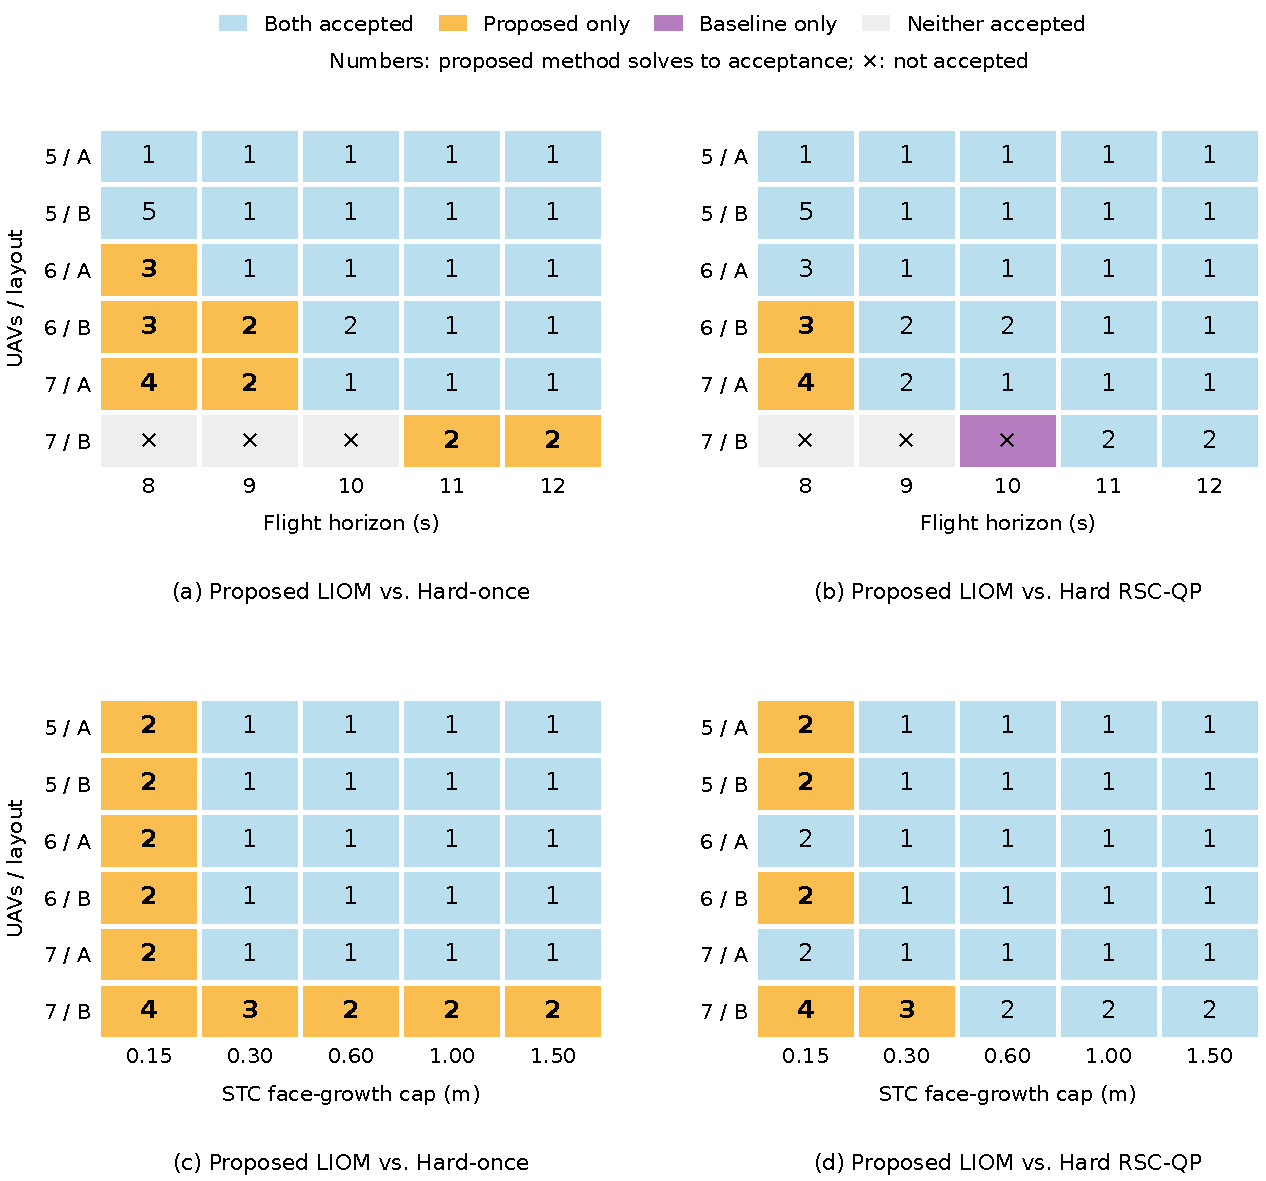
\includegraphics[width=\fulllength]{figures_rest/pressure_sweep.pdf}
\caption{Acceptance across the pressure grids. The upper row varies flight time; the lower row varies spatial-box freedom. A/B denote the two geometric realizations. Colors compare Proposed LIOM with each indicated baseline. Numbers give the proposed method's solves to acceptance; a cross marks its unaccepted attempt.\label{fig:pressure}}
\end{adjustwidth}
\end{figure}

The spatial-box sweep more clearly separates the methods: Proposed LIOM accepts 30/30 settings, Hard-once 20/30, and Hard RSC-QP 25/30. Ten settings have independently confirmed infeasible initial hard-box problems and are recovered in two to four solves. At the smallest cap, every layout requires recovery. All five Hard RSC-QP failures are accepted by the proposed method. Once a hard local region excludes the admissible motion, the low cost of its QP alone offers no route forward. The proposed procedure instead uses intermediate candidates to relocate the corridors while preserving flight time, endpoints, and physical bounds.

The maximum observed wall times among accepted Proposed LIOM runs are 8.51 s in the time sweep and 2.03 s in the box sweep. The seven-UAV B reference exceeds the scalar timing limit at 8 s; at 9 and 10 s, numerical recovery is reached, but the reconstructed outputs do not pass the componentwise motion checks within the stopping budget.

Together, the sweeps demonstrate recovery across multiple layouts and degrees of local restriction. Compatible initial geometry permits a short hard-corridor solve. When that compatibility is lost, the complete recovery procedure provides intermediate candidates for geometry updates and subsequent acceptance at the unchanged flight horizon.
